
\subsection{Focus Area - Communal-Value}
\textbf{Goal:} Identify if a project is valuable to its community of users (including downstream projects) or contributors.
\begin{table}[ht!]
    \centering
    \begin{tabular}{|p{0.35\linewidth} | p{0.6\linewidth}|}
        \hline
        \hfil \textbf{Metric}  & \hfil \textbf{Question} \\
        \hline
		Project Popularity & How popular is an open source project? \\ 
		\hline
		Project Velocity & What is the development speed for an organization? \\ 
		\hline
		Social Listening & How does one measure the value of community interactions and accurately gauge “reputation” of a community as evident from qualitative sentiment? \\ 
		\hline
    \end{tabular}
\end{table}

\hypertarget{project-popularity}{%
\subsubsection{Project Popularity}\label{project-popularity}}

Question: How popular is an open source project?

\hypertarget{description}{%
\paragraph{Description}\label{description}}

Project popularity can be measured by how much activity is visible
around a project. Popularity has a positive feedback loop in which more
popular projects get more attention, attract more users or developers,
and see increases in popularity, spinning the popularity wheel.

Project popularity may be used as a proxy for understanding project
value because open source project economic value is hard to measure, due
to a lack of available usage or sales information for open source
projects.

\hypertarget{objectives}{%
\paragraph{Objectives}\label{objectives}}

In a quest to earn a living wage, and to maximize future employment
opportunities, workers may be interested in knowing which projects are
growing and are underserved. Similarly, from an organizational
perspective, knowing which projects are highly used can be helpful in
knowing which projects might be worth investing in. The Project
Popularity metric can be used to identify the trajectory of a project's
development.

\hypertarget{implementation}{%
\paragraph{Implementation}\label{implementation}}

The project popularity metric is often considered with changes over
time. There are numerous example vectors to consider when measuring
project popularity based on the number of:

\begin{enumerate}
\def\labelenumi{\arabic{enumi}.}
\tightlist
\item
  Social media mentions
\item
  Forks
\item
  \href{https://chaoss.community/metric-change-requests/}{Change
  requests}
\item
  \href{https://chaoss.community/metric-issues-new/}{New Issues}
\item
  Stars, badges, likes
\item
  \href{https://chaoss.community/metric-new-contributors/}{New
  contributors}
\item
  \href{https://chaoss.community/metric-organizational-diversity/}{Organizational
  Diversity}
\item
  Job postings requesting skills in project
\item
  Conversations within and outside of project
\item
  Clones
\item
  Followers
\item
  Downstream dependencies
\item
  People attending events that focus on a project
\end{enumerate}

\hypertarget{visualizations}{%
\subparagraph{Visualizations}\label{visualizations}}

Issues and reviews (change requests) visualization from Cauldron
(GrimoireLab):

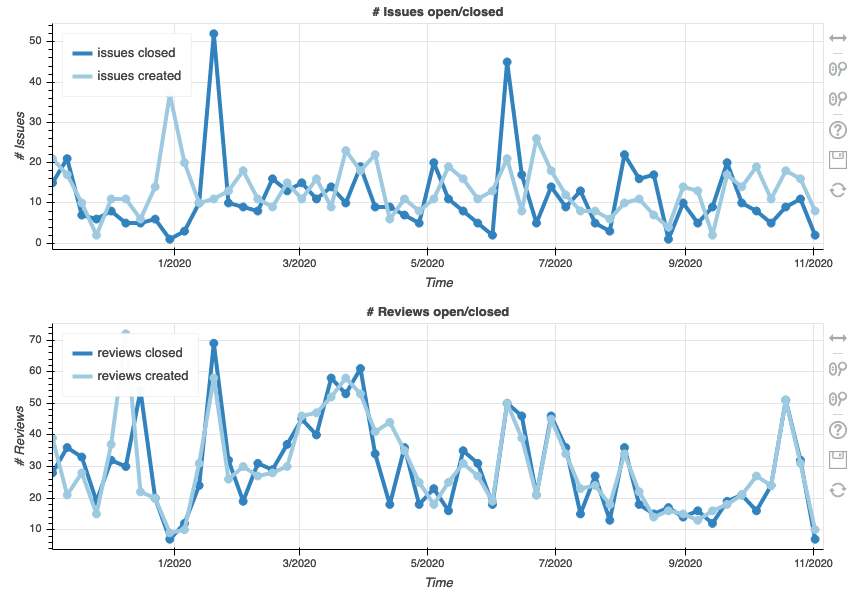
\includegraphics{images/project-popularity_issues-and-reviews.png}

Kubernetes project popularity statistics from DevStats:

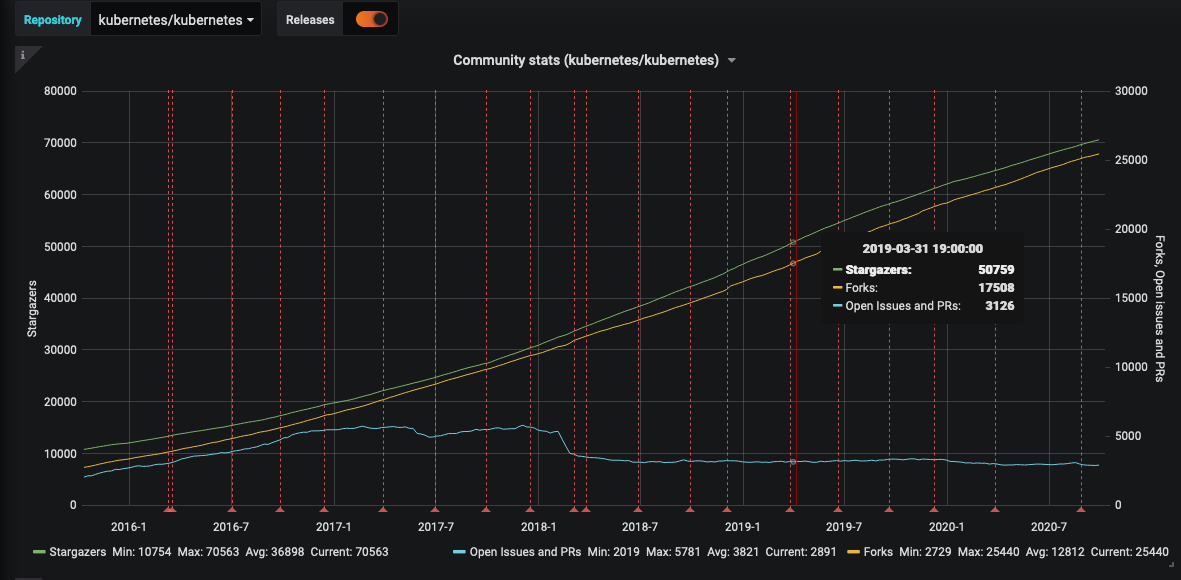
\includegraphics{images/project-popularity_kubernetes.png}

\hypertarget{tools-providing-the-metric}{%
\subparagraph{Tools Providing the
Metric}\label{tools-providing-the-metric}}

\begin{itemize}
\tightlist
\item
  \href{https://github.com/chaoss/augur}{Augur}
\item
  \href{https://chaoss.github.io/grimoirelab/}{GrimoireLab}
\item
  \href{https://cauldron.io/}{Cauldron}
\end{itemize}

\hypertarget{references}{%
\paragraph{References}\label{references}}

\begin{itemize}
\tightlist
\item
  \href{http://blog.honeypot.io/most-exciting-open-source-projects-2018/}{Popular
  OpenSource Projects}
\item
  \href{https://isitmaintained.com/}{Is It Maintained?}
\item
  \href{https://github.blog/2018-02-08-open-source-project-trends-for-2018/}{Open
  Source Project Trends}
\item
  \href{https://www.payscale.com/research/US/Skill=Kubernetes/Salary}{Kubernetes
  Salary}
\end{itemize}
 
\hypertarget{project-velocity}{%
\subsubsection{Project Velocity}\label{project-velocity}}

Question: What is the development speed for an organization?

\hypertarget{description}{%
\paragraph{Description}\label{description}}

Project velocity is the number of issues, the number of pull requests,
volume of commits, and number of contributors as an indicator of
'innovation'.

\hypertarget{objectives}{%
\paragraph{Objectives}\label{objectives}}

Gives an Open Source Program Office (OSPO) manager a way to compare the
project velocity across a portfolio of projects.

The OSPO manager can use the Project Velocity metric to:

\begin{itemize}
\tightlist
\item
  Report project velocity of open source projects vs in-house projects
\item
  Compare project velocity across a portfolio of projects
\item
  Identify which projects grow beyond internal contributors (when
  filtering internal vs. external contributors)
\item
  Identify promising areas in which to get involved
\item
  Highlight areas likely to be the successful platforms over the next
  several years
\end{itemize}

\href{https://www.cncf.io/blog/2017/06/05/30-highest-velocity-open-source-projects}{See
Example}

\hypertarget{implementation}{%
\paragraph{Implementation}\label{implementation}}

Base metrics include:

\begin{itemize}
\tightlist
\item
  \href{https://github.com/chaoss/wg-evolution/blob/master/metrics/Issues_Closed.md}{issues
  closed}
\item
  \href{https://github.com/chaoss/wg-evolution/blob/master/metrics/Reviews.md}{number
  of reviews}
\item
  \href{https://github.com/chaoss/wg-evolution/blob/master/metrics/Code_Changes.md}{\#
  of code changes}
\item
  \href{https://github.com/chaoss/wg-risk/blob/master/metrics/Committers.md}{\#
  of committers}
\end{itemize}

\hypertarget{filters}{%
\subparagraph{Filters}\label{filters}}

\begin{itemize}
\tightlist
\item
  Internal vs external contributors
\item
  Project sources (e.g., internal repositories, open-source
  repositories, and competitor open-source repositories)
\item
  Time
\end{itemize}

\hypertarget{visualizations}{%
\subparagraph{Visualizations}\label{visualizations}}

\begin{itemize}
\tightlist
\item
  X-Axis: Logarithmic scale for Code Changes
\item
  Y-Axis: Logarithmic scale of Sum of Number of Issues and Number of
  Reviews
\item
  Dot-size: Committers
\item
  Dots are projects
\end{itemize}

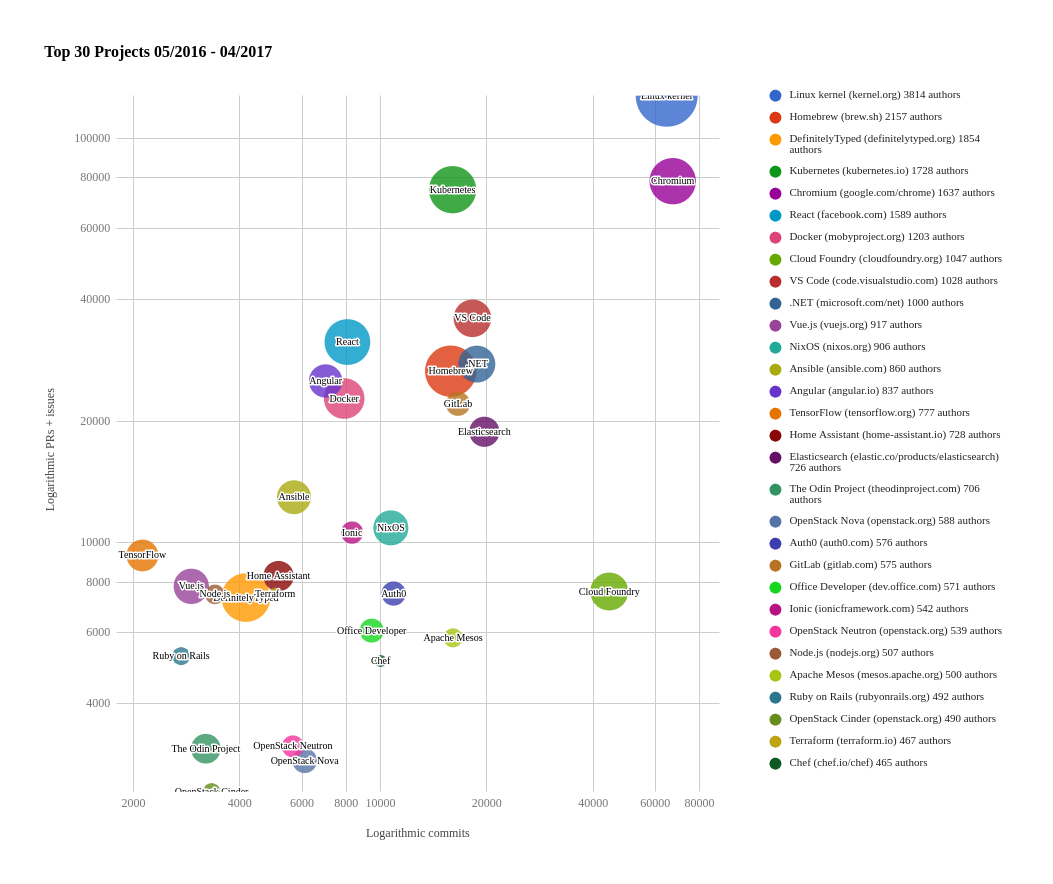
\includegraphics{images/project-velocity_visualization.png}

\href{https://www.cncf.io/blog/2017/06/05/30-highest-velocity-open-source-projects/}{From
CNCF}

\hypertarget{tools-providing-the-metric}{%
\subparagraph{Tools providing the
Metric}\label{tools-providing-the-metric}}

\begin{itemize}
\tightlist
\item
  CNCF -
  \href{https://github.com/cncf/velocity}{https://github.com/cncf/velocity}
\end{itemize}

\hypertarget{references}{%
\paragraph{References}\label{references}}

\begin{itemize}
\tightlist
\item
  \href{https://www.threefivetwo.com/blog/can-open-source-innovation-work-in-the-enterprise}{Can
  Open Source Innovation work in the Enterprise?}
\item
  \href{https://www.nearform.com/blog/want-a-high-performing-culture-make-way-for-open-innovation}{Open
  Innovation for a High Performance Culture}
\item
  \href{https://www.cio.com/article/3213146/open-source-is-powering-the-digital-enterprise.html}{Open
  Source for the Digital Enterprise}
\item
  \href{https://www.cncf.io/blog/2017/06/05/30-highest-velocity-open-source-projects}{Highest
  Velocity Open Source Projects}
\end{itemize}
 
\hypertarget{social-listening}{%
\subsubsection{Social Listening}\label{social-listening}}

Question: How does one measure the value of community interactions and
accurately gauge ``reputation'' of a community as evident from
qualitative sentiment?

\emph{Note: This metric synthesizes several other metrics that can be
derived from trace data, and several process-oriented metrics. Embedded
footnotes annotate areas planned for later clarification, and questions
for later resolution.}

\hypertarget{description}{%
\paragraph{Description}\label{description}}

Social Listening is a combination of
\href{https://blog.hubspot.com/service/social-listening}{social
listening} practices across multiple channels along with a meaningful
set of categorizations. The combination of these tactics can lead to
systematic community analysis and can inform a community strategy that
leads to measurable business value. {[}1{]}

\textbf{Theory and Origin}

Social currency or social capital is a social scientific theory. It
broadly considers how human interactions build relationships and trust
in a community. The Social Listening metric represents the reputation of
a community as measured via community trust, transparency, utility,
consistency, and merit.

Interpersonal relationships are the social fabric of communities. This
is shown in the
\href{https://theadminzone.com/ams/levingers-stage-theory.1272/}{Levinger's
Relationship Model} and
\href{https://psycnet.apa.org/record/1973-28661-000}{Social Penetration
Theory}. Community members' sense of personal and group identity grows
as they interact. Members build shared values, accumulate a sense of
trust, encourage cooperation, and garner reciprocity through acts of
\href{https://en.wikipedia.org/wiki/Self-disclosure}{self-disclosure}.
These interactions build an increased and measurable sense of
connection. The measure of these characteristics is called social
currency. {[}2{]}

\textbf{Results}

The Social Listening metric is a way to sort through a fire hose of
qualitative data from community interactions. A central premise of this
approach is that community members' interactions have an impact on the
community. The Social Listening metric continually measures the
sentiment {[}3{]} from those interactions. It illustrates the reputation
and level of trust between community members and leaders. {[}4{]}

\hypertarget{objectives}{%
\paragraph{Objectives}\label{objectives}}

Analyze the qualitative comments in community interactions. Gain an
overview of sentiment in a community. Get metrics that show at a glance
how a community is and was doing. Use lead metrics from continuous
measurements for proactive community strategy development. Instill trust
in community members that their thoughts and opinions are valued.

\hypertarget{implementation}{%
\paragraph{Implementation}\label{implementation}}

The Social Listening requires the collection of community comments
(communication traces), the definition of a codex, and the on-going
review of the communication traces. {[}5{]}

Set up a Data Collection Platform of your choice as described in the
``Tools'' section below. Ensure it has a minimum of 4 dimensions and 3
communication channels. Once it is set up, the following method is used
to collect, analyze, and interpret results:

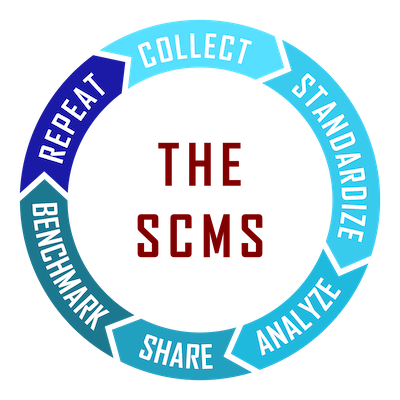
\includegraphics{images/social-listening_circle2.png}

\begin{enumerate}
\def\labelenumi{\arabic{enumi}.}
\item
  \textbf{Collect Communication Traces} -\/- Identify online platforms
  that your community is communicating on. Set up data funnels from the
  primary platform to your Social Listening tool. The critical data for
  the system is user generated content.
\item
  \textbf{Standardize How Communication Traces Should Be Assessed} -\/-
  Use a codex to define important concepts as a ``tracking keyword'' or
  ``category'' in the focal community. This unified codex of terms
  ensures consistent analysis as different people read and tag community
  sentiment. Formalizing the revision and addition structure to this
  codex on a regular basis is a must. {[}5{]}
\item
  \textbf{Analyze the Communication Traces} -\/- Community sentiment is
  analyzed in the Social Listening tool by tagging data with codex
  terms. If the tagging is done by a team of people, it is recommended
  that everyone gets together regularly to discuss trends and ensure
  consistent tag use. If the tagging is done by an artificial
  intelligence algorithm, then a human team should supervise and retrain
  the AI as necessary. {[}5{]}
\item
  \textbf{Share and Visualize the Aggregated Analysis} -\/- Visualize
  the quantitative count of codex terms over time, e.g., in a dashboard.
  This is where the qualitative analysis results produce an easy to
  observe dashboard of trends. Share analysis with team members. {[}6{]}
\item
  \textbf{Benchmark, Set Goals \& Predict Future Growth} -\/- After
  getting enough data to form a benchmark, take stock of where your
  community stands. What are its strengths and weaknesses? What actions
  can be taken to make the community healthier and more robust? Then
  form community initiatives with well-defined goals and execute on
  these projects to affect the social currency metrics for next week.
  {[}6{]}
\item
  \textbf{Repeat the Process} -\/- In regular evaluation meetings,
  discuss the shortcomings of the dataset or collection methods. Come up
  with methods to address these shortcomings in the future. Work
  solutions into the system and move forward. Truth is in the trend,
  power is in the pattern. {[}7{]}
\end{enumerate}

\hypertarget{filters}{%
\subparagraph{Filters}\label{filters}}

\begin{enumerate}
\def\labelenumi{\arabic{enumi}.}
\tightlist
\item
  \textbf{Channel}: Sort by where the data was collected from.
\item
  \textbf{Tag}: Show data based on what codex tags were used to identify
  sentiment in comments.
\item
  \textbf{Time}: Show trends in the data over time and pull specific
  data-sets.
\item
  \textbf{Most impactful comments}: Sort and filter by flags that can be
  placed in the data to highlight specific data points and explain their
  importance.
\item
  \textbf{AI vs. Human tagged}: Filter by whether tags were applied
  programmatically or by a person.
\item
  \textbf{Weighted currency:} Weight the ``importance'' of certain
  comments based on any one individually selected criteria. A resulting
  weighted view is simply a re-order of information based on weight.
\end{enumerate}

\hypertarget{visualizations}{%
\subparagraph{Visualizations}\label{visualizations}}

\textbf{Dashboard visualizing the aggregate metrics:}

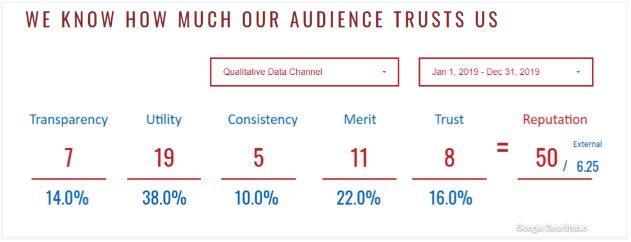
\includegraphics{images/social-listening_dashboard.png}

\textbf{Example Social Listening tool:} On the left, raw community
comments are shown and tags are added in columns immediately to the
right. On the right, a pivot table shows in numbers how often tags
occurred in combination with other tags.

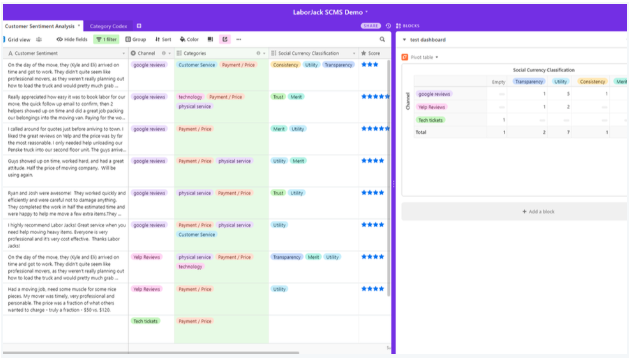
\includegraphics{images/social-listening_tool-example.png}

\textbf{Expanded comments view:} remove the ``quantitative'' from the
fields and provide the best possible way to read the different comments.

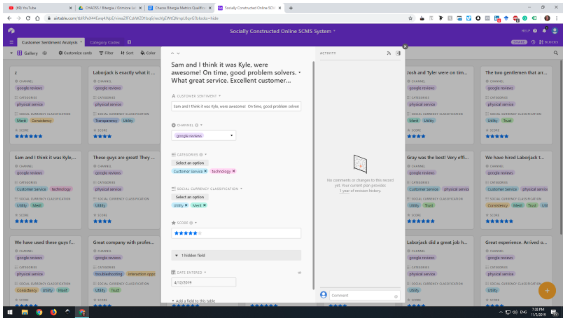
\includegraphics{images/social-listening_expanded-comment.png}

\hypertarget{tools-providing-the-metric}{%
\subparagraph{Tools Providing the
Metric}\label{tools-providing-the-metric}}

To implement the metric any MySQL, smart-sheet, excel, or airtable-like
excel datasheet program works fine. This data should be simplified
enough to interact with other data interfaces to ensure that data
migration is simple, straightforward, and can be automated (such as
google data studio). This requires that systems used to implement the
Social Listening metric work with CSV and other spreadsheet files, and
we heavily recommend open source programs for its implementation.

Once you have this, create a data set with the following data points:
{[}8{]}

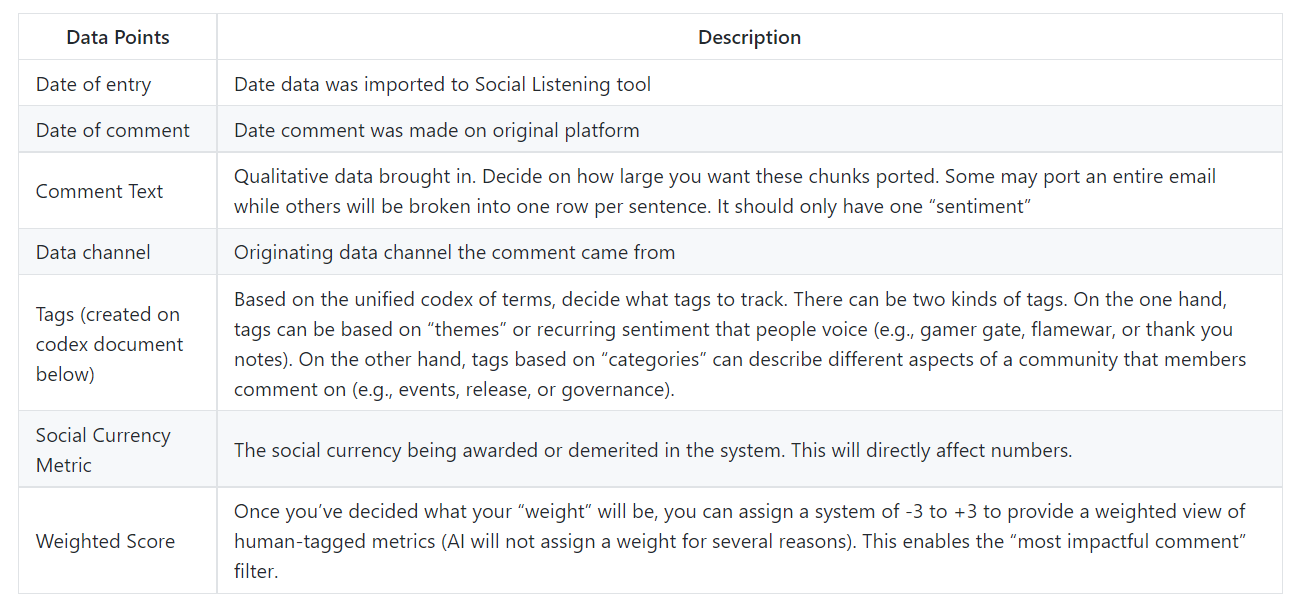
\includegraphics{images/social-listening_data-points-table.png}

Create a second sheet for the Unified Codex of Terms which will define
terms. It should look like this: {[}8{]}

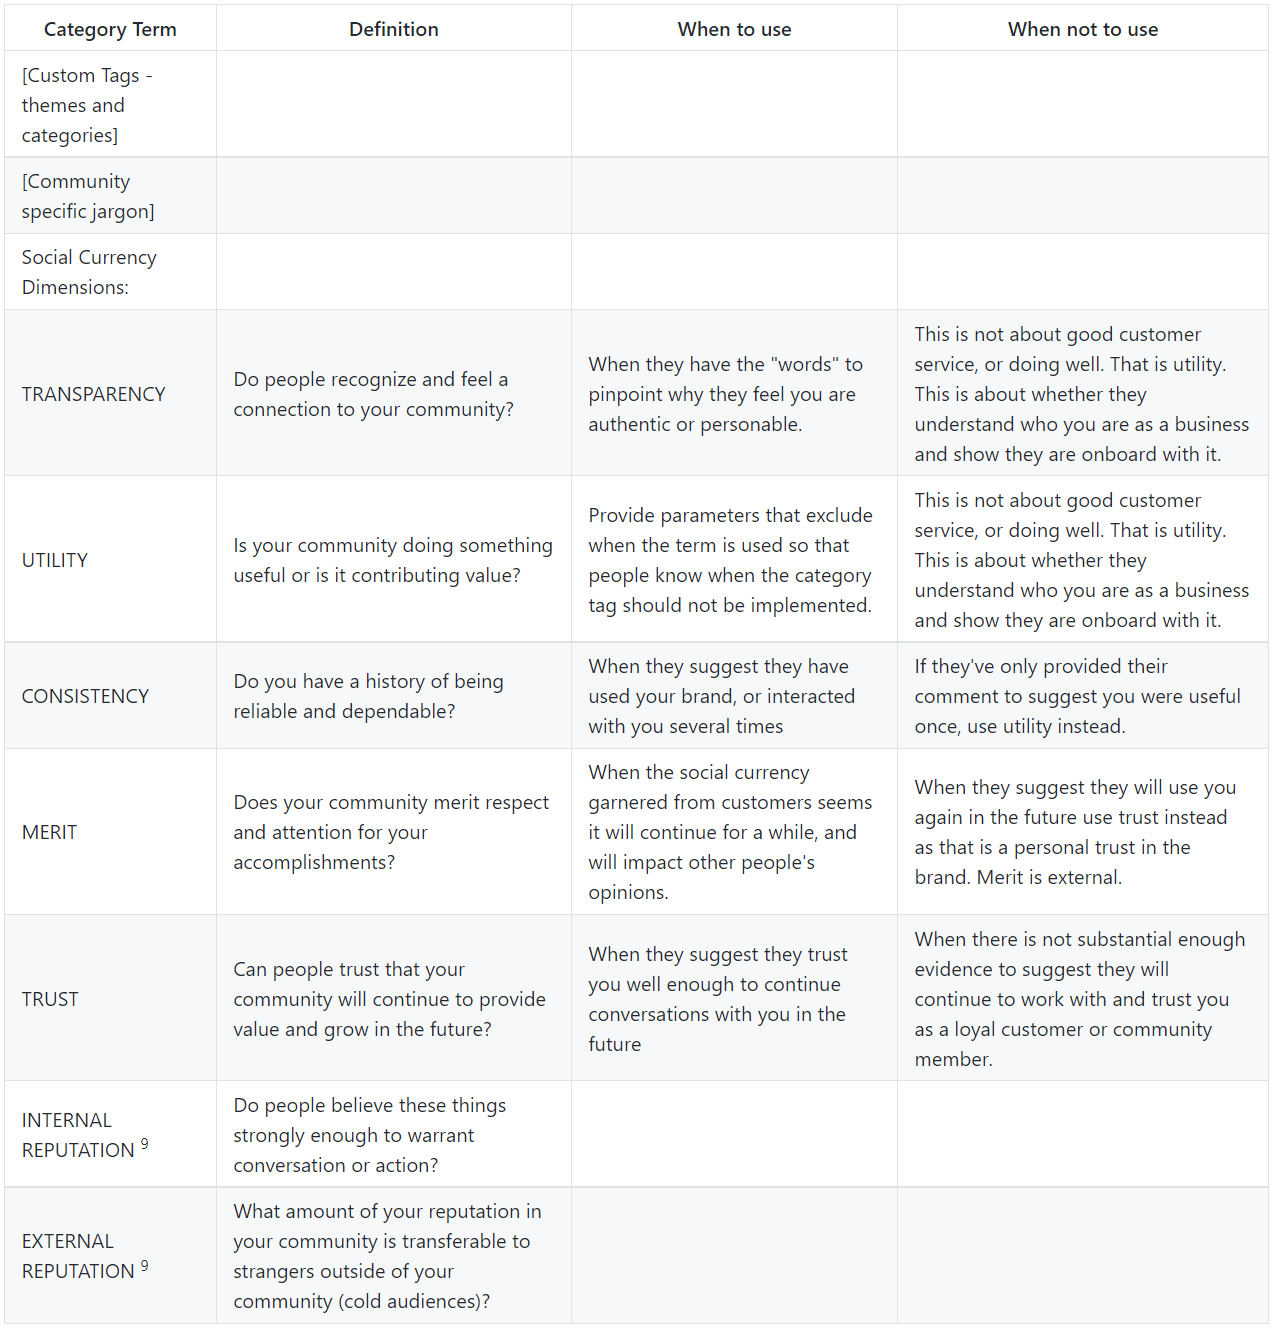
\includegraphics{images/social-listening_unified-codex-terms-table.png}

The codex is filled in by stakeholders on a regular basis by specific
communities and forms the basis for analysis of the data. This is the
MOST IMPORTANT part. Without this the subjectivity of qualitative data
does not follow the rule of generalization: {[}9{]}

\begin{quote}
``A concept applies to B population ONLY SO FAR AS C limitation.''
\end{quote}

\hypertarget{data-collection-strategies}{%
\subparagraph{Data Collection
Strategies}\label{data-collection-strategies}}

Community member comments are available from trace data. The Social
Listening metric ideally imports the comment text automatically into a
tool for tagging. Trace data can be collected from a communities'
collaboration platforms where members write comments, including
ticketing systems, code reviews, email lists, instant messaging, social
media, and fora.

\textbf{Legal and Regulatory Considerations}

\emph{Points of destruction}: Detailed data is destroyed after \emph{xx}
months has passed. Quantitative calculations are kept for up to 250
weeks per GDPR compliance. Data older than 250 weeks becomes archived
data you cannot manipulate but can see. Users can negotiate the primary
statistic.

\hypertarget{references}{%
\paragraph{References}\label{references}}

\begin{itemize}
\tightlist
\item
  \href{https://airtable.com/invite/l?inviteId=inv8u49VVMtQTrfFU\&inviteToken=c49b1ed3759c5cd736901fd81c9f460f86e8e9f462703c4f85a3bdd7250ca5a7}{An
  example implementation on airtable}
\item
  \href{https://datastudio.google.com/open/1X9UdQz8FtHHmjMBpjba3pFqE55lNpwg5}{An
  example implementation in data studio} (report)
\item
  \href{https://datastudio.google.com/open/1Z4EJ03898lZxm2NZVULaEoLS0bYqL79A}{An
  example implementation in data studio} (data source)
\item
  \href{https://drive.google.com/open?id=1zi3JE0bwfEdRdc-wQEZn8GaB7sE8IvxeSeqvVywKnXw}{An
  example implementation in google sheets}
\item
  \href{https://docs.google.com/document/d/1RlAedRBQbhq0oYMCB3VqdawOCZE2XT5R3teydjBZODM/edit\#heading=h.8hyunaadfriq}{Implementation
  documentation} (starts on page 33)
\end{itemize}

\hypertarget{annotated-footnotes}{%
\paragraph{Annotated Footnotes}\label{annotated-footnotes}}

{[}1{]} CHAOSS metrics historically is to create standard definitions
that can be used reliably across projects to support comparisons. This
metric may evolve into a project in the future.

{[}2{]} What metrics emerge from this description? Likely included are:
1. community trust, 2. transparency, 3. utility, 4. consistency, and 5.
merit

{[}3{]} Analysis of sentiment suggests that metric (6) is likely
"Communications Sentiment", and the definition may need to include
references to common sentiment analysis tools, sometimes called "bags of
words".

{[}4{]} Measuring how trust trust is instilled in community members,
such that their thoughts and opinions are valued is likely metric (7)
that will define a process, and perhaps is not measurable via trace
data.

{[}5{]} A substantial portion of any codex for open source software will
be common across projects, and each project is likely to have a set of
particular interests that are a subset of that codex. In some cases,
their main interests may not be present in an established codex
component. In general, the codex, like the CHAOSS project itself, is
open sourced as shared metadata to ensure shared understanding across
open source communities.

{[}6{]} This describes the evolution of a standard codex, and its
elements through the process of CHAOSS working groups and projects,
characterized in the previous footnote. Likely this will be a process
metric (8).

{[}7{]} Candidate process oriented metric (9).

{[}8{]} Examples of data coded using the open sourced codex, as it
evolves, will be essential components for advancing open source software
through Social Listening. Implementations will require these examples,
and their provision as open source assets of the CHAOSS project will
return value as shared data.

{[}9{]} Internal and external reputation are likely metrics (10), and
(11) arising from the Social Listening metric.
 
